\chapter{Threat model and site map}\label{kap:Threat model and site map}

\renewcommand{\figurename}{Fig.}


\begin{figure}[H]
    \centering
    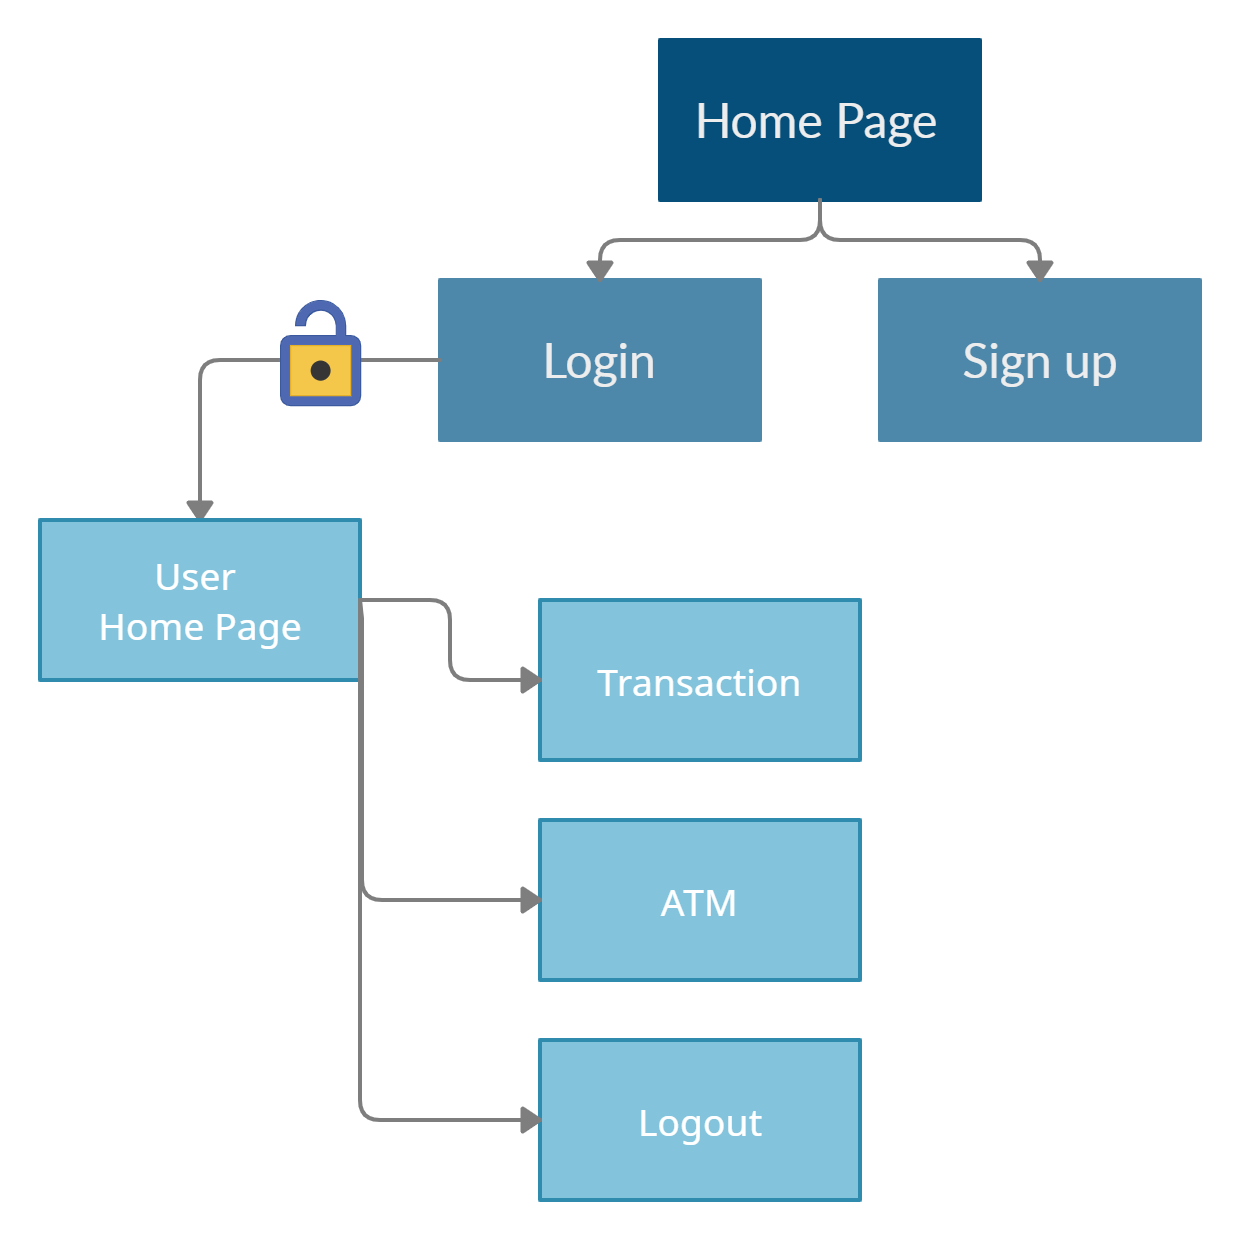
\includegraphics[width=\textwidth]{pics/pic1 Site map.png}
    \caption{Site map}
    \label{fig:kap1fig1sitemap}
\end{figure}

A visitor can only see login and signup pages from the homepage. When an unlogged user tries to visit the URL of any other page, he gets redirected back to the homepage.

\begin{figure}[H]
    \centering
    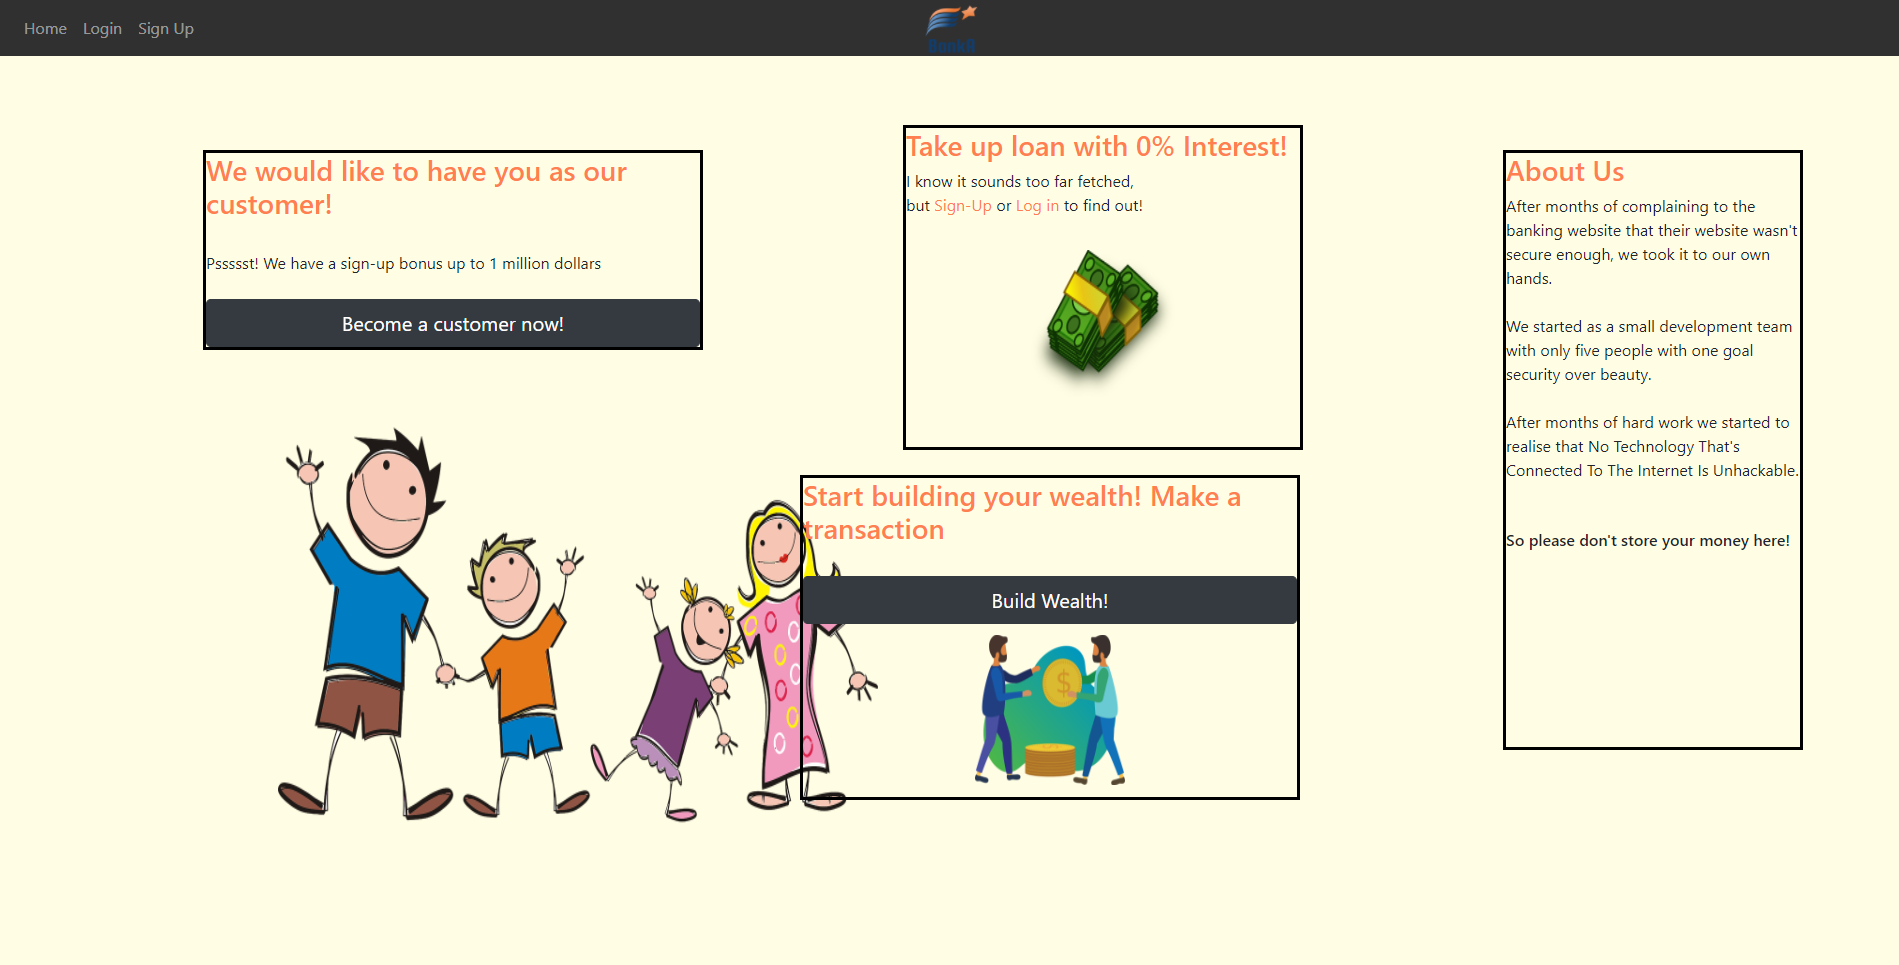
\includegraphics[width=\textwidth]{pics/pic2 home visitor.PNG}
    \caption{Site landing page}
\end{figure}

After logging in, the user gets access to ATM and Transaction pages, also homepage changes to show the user’s balance and transaction history.

\begin{figure}[H]
    \centering
    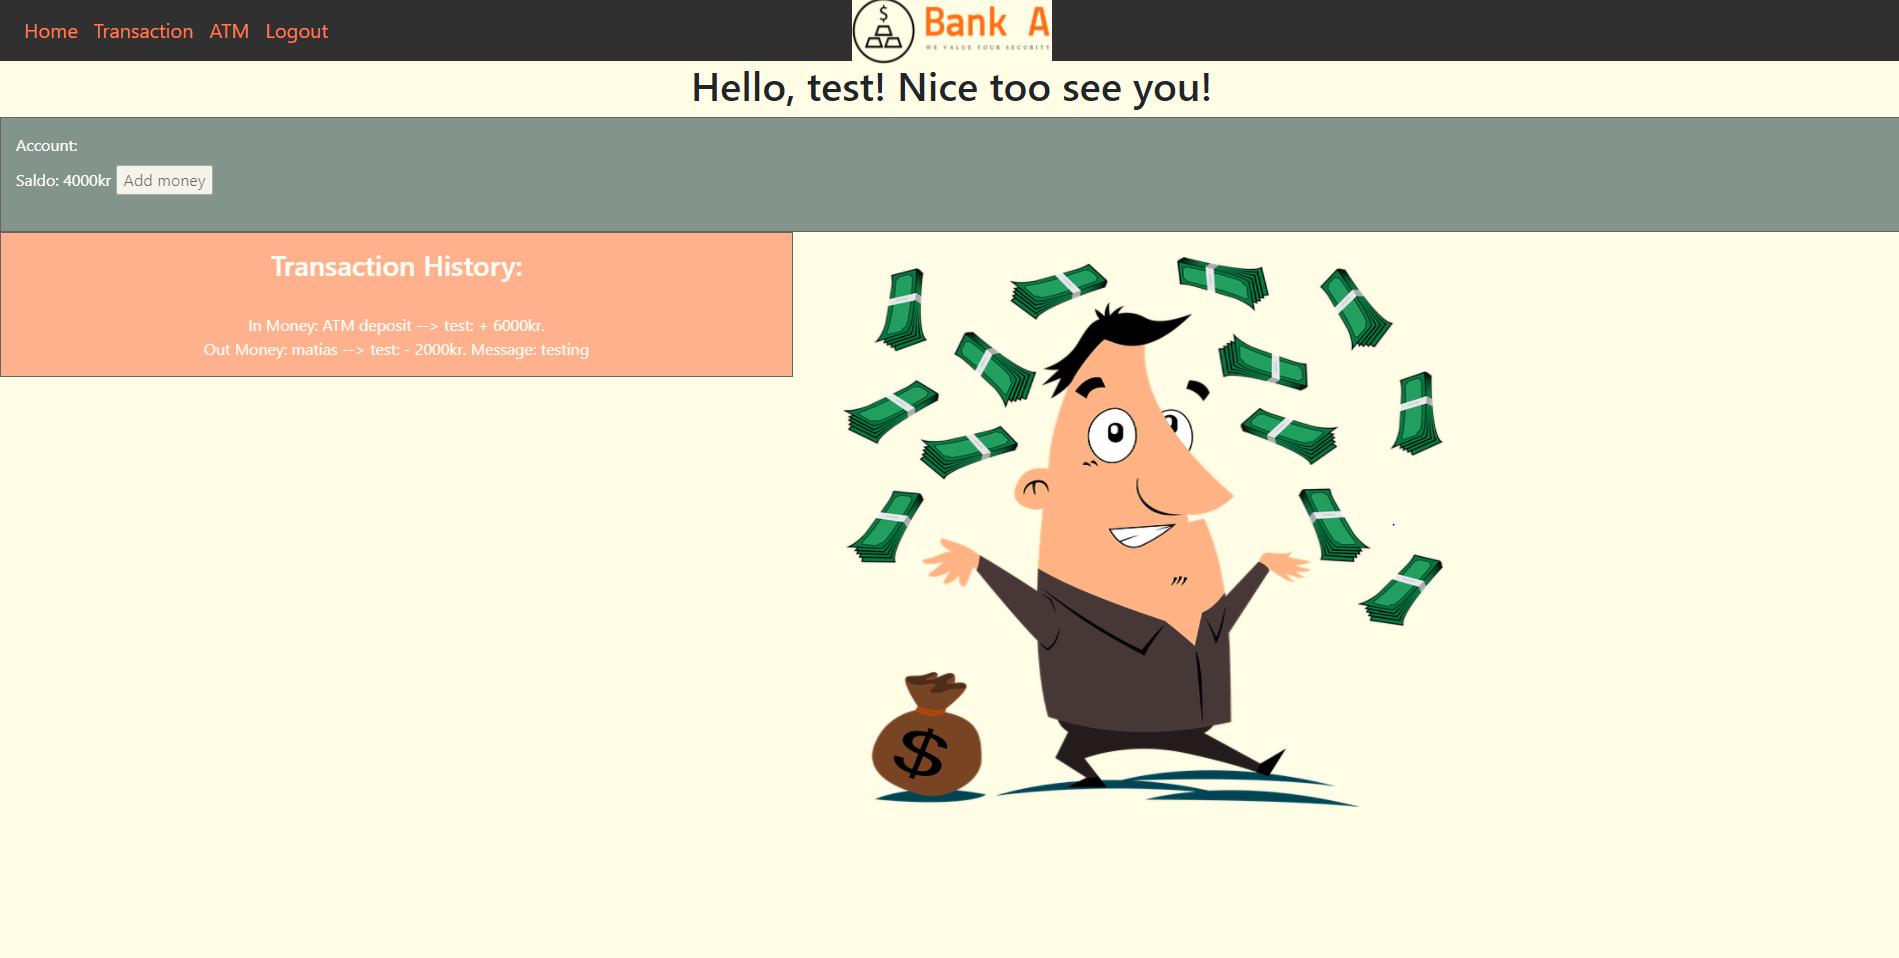
\includegraphics[width=\textwidth]{pics/pic3homeuser.PNG}
    \caption{User homepage}
\end{figure}

\begin{figure}[H]
    \centering
    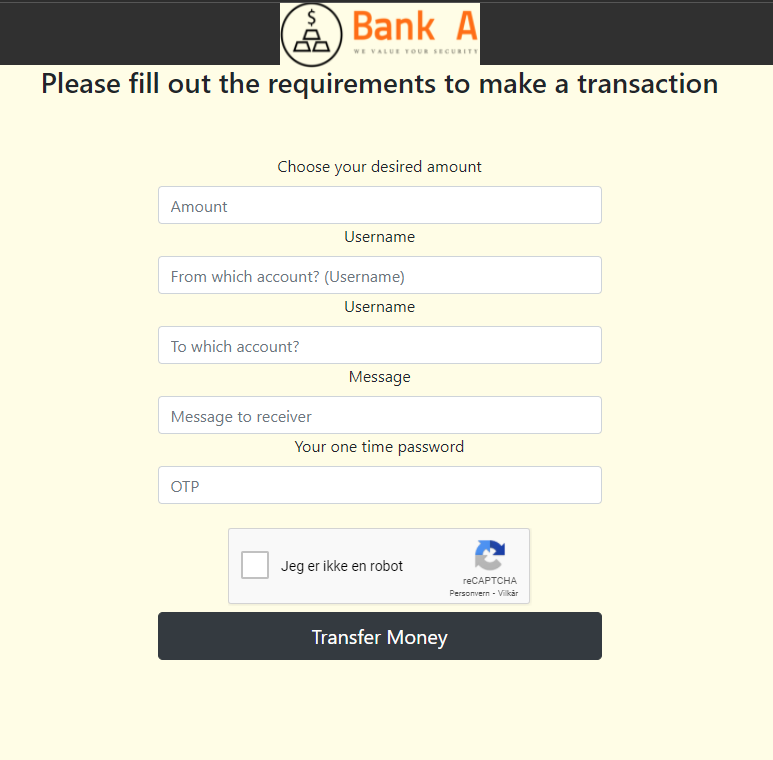
\includegraphics[width=\textwidth]{pics/pic 3.1.PNG}
    \caption{Transaction page}
\end{figure}

To transfer cash from your own bank account in the Transaction page, the user must know the username of the receiver, and in addition confirm his own. The user can also choose to send it with a message. This action must go through reCAPTCHA and 2FA authentication. 

ATM service simulates depositing cash in a local ATM to fill your account. This page looks like this, and must also confirm/verify the name of the user, reCAPTCHA and 2FA authentication. The limit is set to 10 000kr to have realistic values. The ATM page looks like this:

\begin{figure}[H]
    \centering
    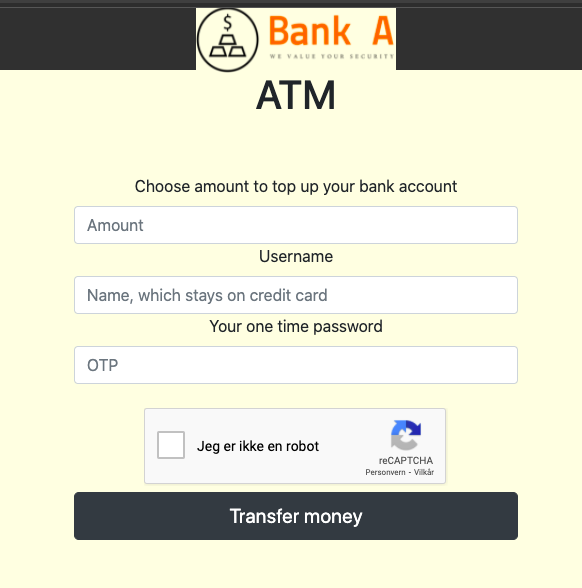
\includegraphics[width=\textwidth]{pics/atmPage.png}
    \caption{ATM page}
\end{figure}